\documentclass{article}
\usepackage[utf8]{inputenc}
\usepackage[usenames,dvipsnames,svgnames]{xcolor}
\usepackage{tikz}
\usepackage{pgfplots}

\usetikzlibrary{shadows}
\usetikzlibrary{shapes}
\usetikzlibrary{decorations}
\tikzset{>=stealth} %% makes all arrows the same
%% Parchment Style
\colorlet{background}{Apricot!7} % Color of the page
\colorlet{textColor}{Sepia!60!black} % Color of the text
\colorlet{penColor}{green!50!black} % Color of a curve in a plot
\colorlet{penColor2}{blue!50!black} % Color of a curve in a plot
\colorlet{fill1}{green!50!black!20} % Color of fill in a plot
\colorlet{fill2}{blue!10} % Color of fill in a plot
\colorlet{gridColor}{gray!30} % Color of grid in a plot
\colorlet{definitionBackground}{Sepia!10!background} % Color of the background of a definition
\colorlet{theoremBackground}{BrickRed!10!background} % Color of the background of a theorem
\colorlet{mainTheoremBorder}{Sepia} % Color of the border of a main theorem
\colorlet{warningBackground}{BrickRed!10!background} % Color of the background of a theorem
\colorlet{cowLight}{background} % the light colors of the cow --
                                % usually the same as the background
\colorlet{cowDark}{textColor} % the dark colors of the cow -- usually

%% Modern Style
\colorlet{background}{Black!7} % Color of the page
\colorlet{textColor}{Black!90} % Color of the text


\colorlet{penColor}{blue!50!black} % Color of a curve in a plot
\colorlet{penColor2}{red!50!black} % Color of a curve in a plot
\colorlet{penColor3}{red!50!blue} % Color of a curve in a plot
\colorlet{penColor4}{green!50!black} % Color of a curve in a plot
\colorlet{penColor5}{orange!80!black} % Color of a curve in a plot
\colorlet{fill1}{blue!50!black!20} % Color of fill in a plot
\colorlet{fill2}{blue!10} % Color of fill in a plot
\colorlet{fillp}{fill1} % Color of positive area
\colorlet{filln}{red!50!black!20} % Color of negative area
\newcommand{\surfaceColor}{violet}
\newcommand{\surfaceColorTwo}{redyellow}
\newcommand{\sliceColor}{greenyellow}
\colorlet{gridColor}{gray!50} % Color of grid in a plot
\colorlet{definitionBackground}{black!8!background} % Color of the background of
                                          % a definition
\colorlet{theoremBackground}{blue!50!black!8!background} % Color of the background of a theorem
\colorlet{mainTheoremBorder}{blue!50!black} % Color of the border of a main theorem
\colorlet{mainOtherBorder}{black} % Color of the border of a main theorem
\colorlet{cowLight}{background} % the light colors of the cow --
                                % usually the same as the background
\colorlet{cowDark}{textColor} % the dark colors of the cow -- usually
                              % the same as the text
\colorlet{hyperColor}{green!30!penColor} % Color of a link

\begin{document}

\begin{figure}[.5in]
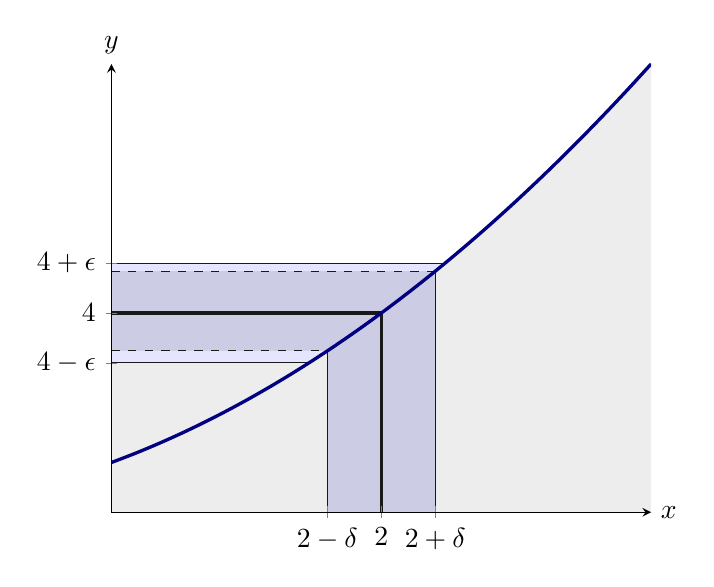
\begin{tikzpicture}
  \begin{axis}[
            domain=1:3,
            axis lines =left, xlabel=$x$, ylabel=$y$,
            every axis y label/.style={at=(current axis.above origin),anchor=south},
            every axis x label/.style={at=(current axis.right of origin),anchor=west},
            xtick={1.8,2,2.2}, ytick={3,4,5},
            xticklabels={$2-\delta$,$2$,$2+\delta$}, yticklabels={$4-\epsilon$,$4$,$4+\epsilon$},
            axis on top,
          ]
          \addplot [color=textColor, fill=fill2, smooth, domain=(1:2.236)] {5} \closedcycle;
          \addplot [color=textColor, dashed, fill=fill1, domain=(1:2.2)] {4.84} \closedcycle;
          \addplot [color=textColor, dashed, fill=fill2, domain=(1:1.8)] {3.24} \closedcycle;
          \addplot [textColor, very thick, smooth, domain=(1:2)] {4};
          \addplot [color=textColor, fill=background, smooth, domain=(1:1.8)] {3} \closedcycle;
    \addplot [draw=none, fill=background, smooth] {x^2} \closedcycle;
          \addplot [fill=fill1, draw=none, domain=1.8:2.2] {x^2} \closedcycle;
          \addplot [textColor, very thick] plot coordinates {(2,0) (2,4)};
          \addplot [textColor] plot coordinates {(1.8,0) (1.8,3.24)};
          \addplot [textColor] plot coordinates {(2.2,0) (2.2,4.84)};
    \addplot [very thick,penColor, smooth] {x^2};
        \end{axis}
\end{tikzpicture}
\label{plot:x^2 lim dfn}
\caption{The $(\epsilon,\delta)$-criterion for $\lim_{x\to 2}
  x^2=4$. Here $\delta= \min\{\frac{\epsilon}{5}, 1 \}$.}
\end{figure}
\end{document}